\documentclass[12pt]{article}
\usepackage{fontspec}
\usepackage{fullpage}
\usepackage{hyperref}
\hypersetup{bookmarks=true,colorlinks=true,linkcolor=red,citecolor=blue,filecolor=magenta,urlcolor=cyan}
\usepackage{amsmath}
\usepackage{amssymb}
\usepackage{mathtools}
\usepackage{unicode-math}
\usepackage{tabu}
\usepackage{longtable}
\usepackage{booktabs}
\usepackage{caption}
\usepackage{graphics}
\usepackage{enumitem}
\usepackage{filecontents}
\usepackage[backend=bibtex]{biblatex}
\usepackage{url}
\setmathfont{Latin Modern Math}
\global\tabulinesep=1mm
\newlist{symbDescription}{description}{1}
\setlist[symbDescription]{noitemsep, topsep=0pt, parsep=0pt, partopsep=0pt}
\bibliography{bibfile}
\title{Software Requirements Specification for Solar Water Heating Systems}
\author{Thulasi Jegatheesan}
\begin{document}
\maketitle
\tableofcontents
\newpage
\section{Reference Material}
\label{Sec:RefMat}
This section records information for easy reference.
\subsection{Table of Units}
\label{Sec:ToU}
The unit system used throughout is SI (Système International d'Unités). In addition to the basic units, several derived units are also used. For each unit, the table lists the symbol, a description and the SI name.
\begin{longtable}{l l}
\toprule
Symbol & Description
\\
\midrule
\endhead
${}^{\circ}$C & temperature (centigrade)
\\
J & energy (joule)
\\
kg & mass (kilogram)
\\
m & length (metre)
\\
s & time (second)
\\
W & power (watt)
\\
\bottomrule
\caption{}
\label{Table:ToU}
\end{longtable}
\subsection{Table of Symbols}
\label{Sec:ToS}
The table that follows summarizes the symbols used in this document along with their units. The choice of symbols was made to be consistent with the heat transfer literature and with existing documentation for solar water heating systems. The symbols are listed in alphabetical order.
\begin{longtabu}{l X[l] l}
\toprule
Symbol & Description & Units
\\
\midrule
\endhead
${A_{C}}$ & Heating coil surface area & $\text{m}^{2}$
\\
${A_{in}}$ & Surface area over which heat is transferred in & $\text{m}^{2}$
\\
${A_{out}}$ & Surface area over which heat is transferred out & $\text{m}^{2}$
\\
$C$ & Specific heat capacity & $\frac{\text{J}}{(\text{kg}{}^{\circ}\text{C})}$
\\
${C^{L}}$ & Specific heat capacity of a liquid & $\frac{\text{J}}{(\text{kg}{}^{\circ}\text{C})}$
\\
${C_{W}}$ & Specific heat capacity of water & $\frac{\text{J}}{(\text{kg}{}^{\circ}\text{C})}$
\\
$D$ & Diameter of tank & m
\\
$E$ & Sensible heat & J
\\
${E_{W}}$ & Change in heat energy in the water & J
\\
$g$ & Volumetric heat generation per unit volume & $\frac{\text{W}}{\text{m}^{3}}$
\\
$h$ & Convective heat transfer coefficient & $\frac{\text{W}}{(\text{m}^{2}{}^{\circ}\text{C})}$
\\
${h_{C}}$ & Convective heat transfer coefficient between coil and water & $\frac{\text{W}}{(\text{m}^{2}{}^{\circ}\text{C})}$
\\
$L$ & Length of tank & m
\\
$m$ & Mass & kg
\\
${m_{W}}$ & Mass of water & kg
\\
$\mathbf{\hat{n}}$ & Normal Vector & --
\\
$q$ & Heat flux & $\frac{\text{W}}{\text{m}^{2}}$
\\
${q_{C}}$ & Heat flux into the water from the coil & $\frac{\text{W}}{\text{m}^{2}}$
\\
${q_{in}}$ & Heat flux input & $\frac{\text{W}}{\text{m}^{2}}$
\\
${q_{out}}$ & Heat flux output & $\frac{\text{W}}{\text{m}^{2}}$
\\
$\mathbf{q}$ & Thermal flux vector & $\frac{\text{W}}{\text{m}^{2}}$
\\
$S$ & Surface & $\text{m}^{2}$
\\
$T$ & Temperature & ${}^{\circ}$C
\\
$t$ & Time & s
\\
$ΔT$ & Change in temperature & ${}^{\circ}$C
\\
${T_{C}}$ & Temperature of the heating coil & ${}^{\circ}$C
\\
${T_{env}}$ & Temperature of the environment & ${}^{\circ}$C
\\
${t_{final}}$ & Final time & s
\\
${T_{init}}$ & Initial temperature & ${}^{\circ}$C
\\
${T_{W}}$ & Temperature of the water & ${}^{\circ}$C
\\
$V$ & Volume & $\text{m}^{3}$
\\
${V_{W}}$ & Volume of water & $\text{m}^{3}$
\\
$π$ & Circumference to diameter ratio & --
\\
$ρ$ & Density & $\frac{\text{kg}}{\text{m}^{3}}$
\\
${ρ_{W}}$ & Density of water & $\frac{\text{kg}}{\text{m}^{3}}$
\\
${τ_{W}}$ & ODE parameter for water & s
\\
$∇$ & Gradient & --
\\
\bottomrule
\caption{}
\label{Table:ToS}
\end{longtabu}
\subsection{Abbreviations and Acronyms}
\label{Sec:TAbbAcc}
\begin{longtable}{l l}
\toprule
Abbreviation & Full Form
\\
\midrule
\endhead
A & Assumption
\\
DD & Data Definition
\\
GD & General Definition
\\
GS & Goal Statement
\\
IM & Instance Model
\\
LC & Likely Change
\\
ODE & Ordinary Differential Equation
\\
PS & Physical System Description
\\
R & Requirement
\\
SRS & Software Requirements Specification
\\
SWHS & Solar Water Heating System
\\
TM & Theoretical Model
\\
UC & Unlikely Change
\\
Uncert. & Typical Uncertainty
\\
\bottomrule
\caption{}
\label{Table:TAbbAcc}
\end{longtable}
\section{Introduction}
\label{Sec:Intro}
Due to increasing cost, diminishing availability, and negative environmental impact of fossil fuels, there is a higher demand for renewable energy sources and energy storage technology. Solar water heating systems provide a novel way of storing energy.
The following section provides an overview of the Software Requirements Specification (SRS) for solar water heating systems. The developed program will be referred to as Solar Water Heating System (SWHS). This section explains the purpose of this document, the scope of the system, the characteristics of the intended reader, and the organization of the document.
\subsection{Purpose of Document}
\label{Sec:DocPurpose}
The main purpose of this document is to describe the modelling of solar water heating system. The goals and theoretical models used in the SWHS code are provided, with an emphasis on explicitly identifying assumptions and unambiguous definitions. This document is intended to be used as a reference to provide ad hoc access to all information necessary to understand and verify the model. The SRS is abstract because the contents say what problem is being solved, but do not say how to solve it.
This document will be used as a starting point for subsequent development phases, including writing the design specification and the software verification and validation plan. The design document will show how the requirements are to be realized, including decisions on the numerical algorithms and programming environment. The verification and validation plan will show the steps that will be used to increase confidence in the software documentation and the implementation. Although the SRS fits in a series of documents that follow the so-called waterfall model, the actual development process is not constrained in any way. Even when the waterfall model is not followed, as Parnas and Clements point out \cite{parnasClements1986}, the most logical way to present the documentation is still to ``fake'' a rational design process.
\subsection{Scope of Requirements}
\label{Sec:ReqsScope}
The scope of the requirements includes thermal analysis of a single solar water heating tank. Given the appropriate inputs, SWHS predicts the temperature and thermal energy histories for the water.
\subsection{Characteristics of Intended Reader}
\label{Sec:ReaderChars}
Reviewers of this documentation should have an understanding of heat transfer theory from level 3 or 4 mechanical engineering and differential equations from level 1 and 2 calculus. The users of SWHS can have a lower level of expertise, as explained in \hyperref[Sec:UserChars]{Section: User Characteristics}.
\subsection{Organization of Document}
\label{Sec:DocOrg}
The organization of this document follows the template for an SRS for scientific computing software proposed by \cite{dParnas1972} and \cite{parnasClements1984}. The presentation follows the standard pattern of presenting goals, theories, definitions, and assumptions. For readers that would like a more bottom up approach, they can start reading the instance models in \hyperref[Sec:IMs]{Section: Instance Models} and trace back to find any additional information they require.
The goal statements (\hyperref[Sec:GoalStmt]{Section: Goal Statements}) are refined to the theoretical models, and the theoretical models (\hyperref[Sec:TMs]{Section: Theoretical Models}) to the instance models (\hyperref[Sec:IMs]{Section: Instance Models}). The instance model to be solved is referred to as \hyperref[IM:eBalanceOnWtr]{IM: eBalanceOnWtr}. The instance model provides the Ordinary Differential Equation (ODE) that model the solar water heating system. SWHS solves this ODE.
\section{General System Description}
\label{Sec:GenSysDesc}
This section provides general information about the system. It identifies the interfaces between the system and its environment, describes the user characteristics, and lists the system constraints.
\subsection{System Context}
\label{Sec:SysContext}
\hyperref[Figure:SysCon]{Fig:SysCon} shows the system context. A circle represents an external entity outside the software, the user in this case. A rectangle represents the software system itself (SWHS). Arrows are used to show the data flow between the system and its environment.
\begin{figure}
\begin{center}
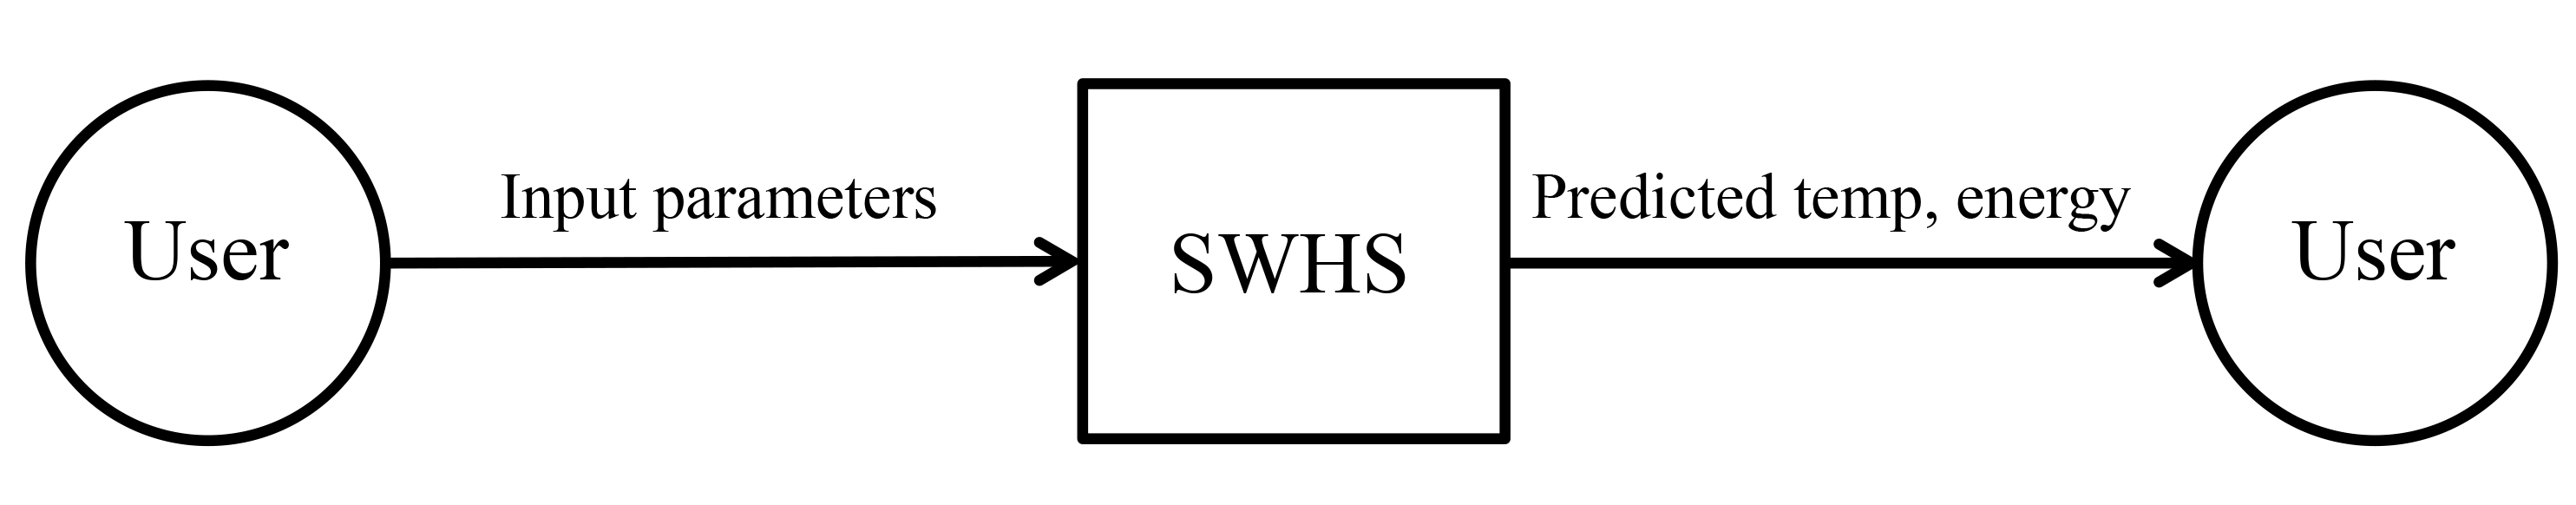
\includegraphics[width=\textwidth]{../../../datafiles/SWHS/SystemContextFigure.png}
\caption{\hyperref[Figure:SysCon]{Fig:SysCon}: System Context}
\label{Figure:SysCon}
\end{center}
\end{figure}
SWHS is mostly self-contained. The only external interaction is through the user interface. The responsibilities of the user and the system are as follows:
\begin{itemize}
\item{User Responsibilities:}
\begin{itemize}
\item{Provide the input data to the system, ensuring no errors in the data entry}
\item{Take care that consistent units are used for input variables}
\end{itemize}
\item{SWHS Responsibilities:}
\begin{itemize}
\item{Detect data type mismatch, such as a string of characters instead of a floating point number}
\item{Determine if the inputs satisfy the required physical and software constraints}
\item{Calculate the required outputs}
\end{itemize}
\end{itemize}
\subsection{User Characteristics}
\label{Sec:UserChars}
The end user of SWHS should have an understanding of undergraduate Level 1 Calculus and Physics.
\subsection{System Constraints}
\label{Sec:SysConstraints}
There are no system constraints.
\section{Specific System Description}
\label{Sec:SpecSystDesc}
This section first presents the problem description, which gives a high-level view of the problem to be solved. This is followed by the solution characteristics specification, which presents the assumptions, theories, and definitions that are used.
\subsection{Problem Description}
\label{Sec:ProbDesc}
SWHS is a computer program developed to investigate the heating of water in a solar water heating tank.
\subsubsection{Terminology and Definitions}
\label{Sec:TermDefs}
This subsection provides a list of terms that are used in the subsequent sections and their meaning, with the purpose of reducing ambiguity and making it easier to correctly understand the requirements.
\begin{itemize}
\item{Heat flux: The rate of thermal energy transfer through a given surface per unit time}
\item{Specific heat capacity: The amount of energy required to raise the temperature of the unit mass of a given substance by a given amount}
\item{Thermal conduction: The transfer of heat energy through a substance}
\item{Transient: Changing with time}
\end{itemize}
\subsubsection{Physical System Description}
\label{Sec:PhysSyst}
The physical system of SWHS, as shown in \hyperref[Figure:Tank]{Fig:Tank}, includes the following elements:
\begin{itemize}
\item[PS1:]Tank containing water.
\item[PS2:]Heating coil at bottom of tank. (${q_{C}}$ represents the heat flux into the water from the coil.)
\end{itemize}
\begin{figure}
\begin{center}
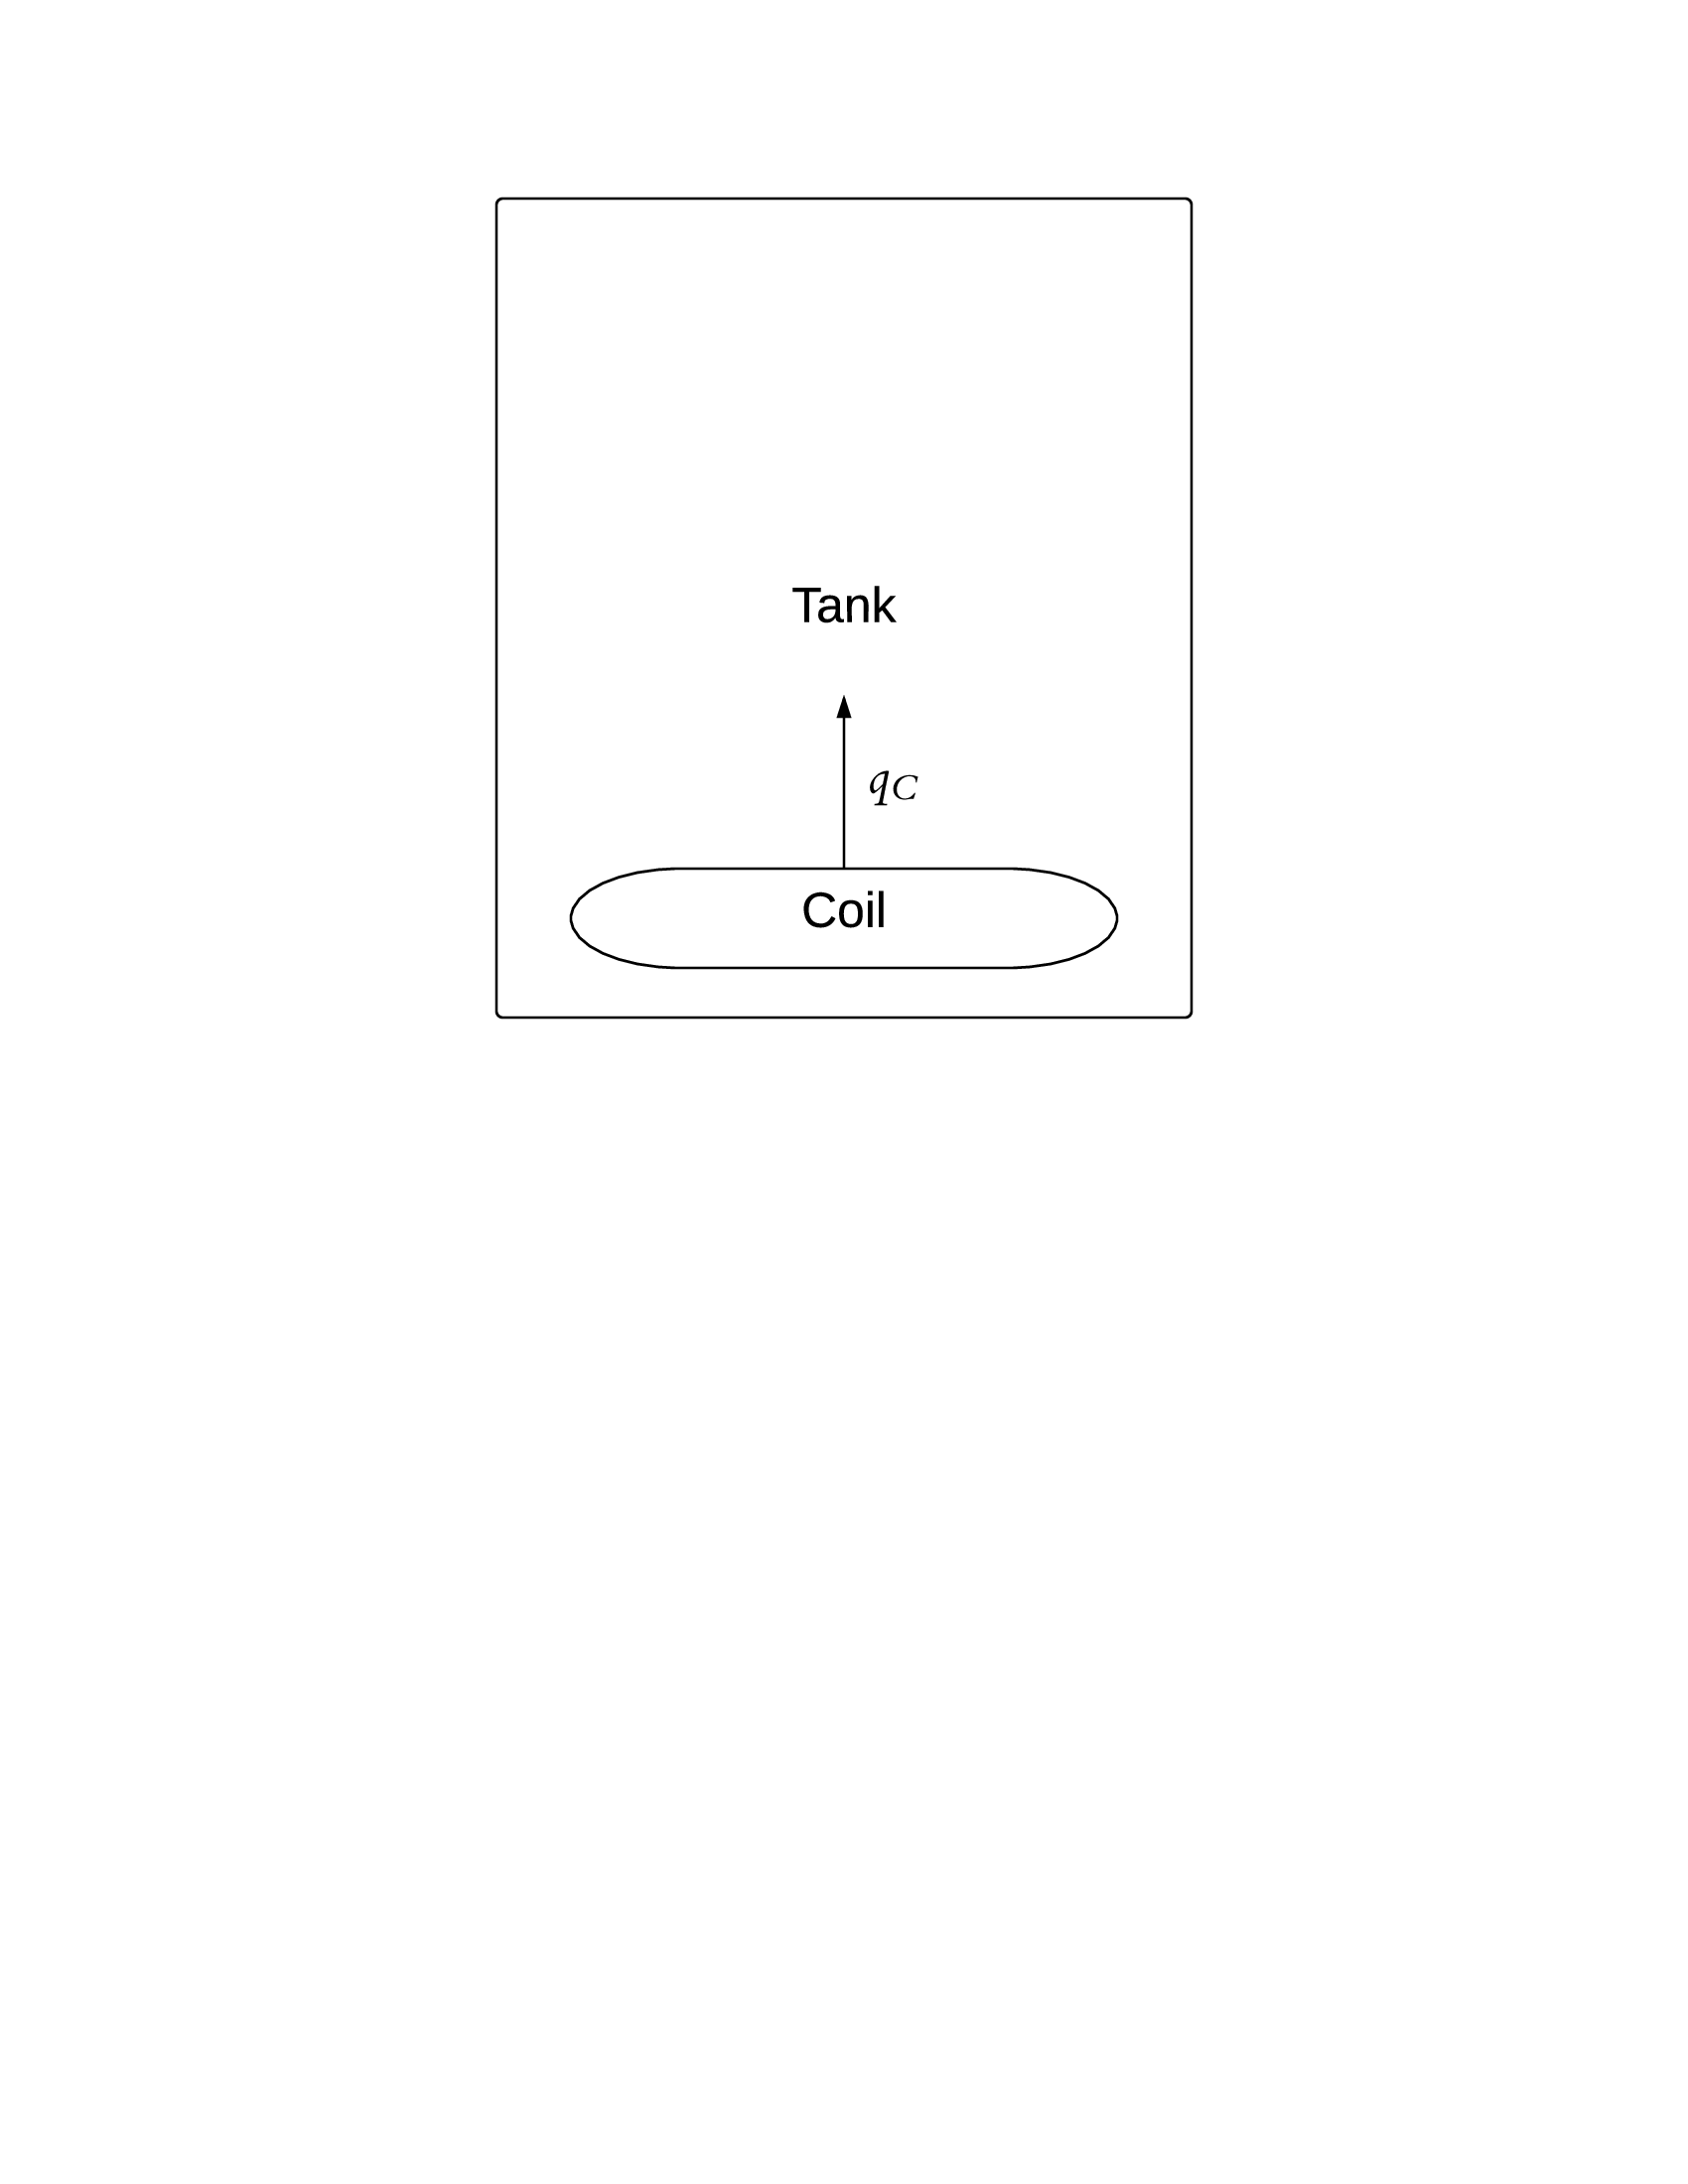
\includegraphics[width=\textwidth]{../../../datafiles/NoPCM/TankWaterOnly.png}
\caption{Solar water heating tank, with heat flux from heating coil of ${q_{C}}$}
\label{Figure:Tank}
\end{center}
\end{figure}
\subsubsection{Goal Statements}
\label{Sec:GoalStmt}
Given the temperature of the heating coil, the initial temperature of the water, and the material properties, the goal statements are:
\begin{itemize}
\item[Predict-Water-Temperature:\phantomsection\label{waterTempGS}]Predict the temperature of the water over time.
\item[Predict-Water-Energy:\phantomsection\label{waterEnergyGS}]Predict the change in heat energy in the water over time.
\end{itemize}
\subsection{Solution Characteristics Specification}
\label{Sec:SolCharSpec}
The instance models that govern SWHS are presented in \hyperref[Sec:IMs]{Section: Instance Models}. The information to understand the meaning of the instance models and their derivation is also presented, so that the instance models can be verified.
\subsubsection{Assumptions}
\label{Sec:Assumps}
This section simplifies the original problem and helps in developing the theoretical model by filling in the missing information for the physical system. The numbers given in the square brackets refer to the Theoretical Models \hyperref[Sec:TMs]{Section: Theoretical Models}, General Definitions \hyperref[Sec:GDs]{Section: General Definitions}, Data Definitions \hyperref[Sec:DDs]{Section: Data Definitions}, Instance Models \hyperref[Sec:IMs]{Section: Instance Models}, Likely Changes \hyperref[Sec:LCs]{Section: Likely Changes}, or Unlikely Changes \hyperref[Sec:UCs]{Section: Unlikely Changes}, in which the respective assumption is used.
\begin{itemize}
\item[Thermal-Energy-Only:\phantomsection\label{assumpTEO}]The only form of energy that is relevant for this problem is thermal energy. All other forms of energy, such as mechanical energy, are assumed to be negligible. \hyperref[TM:consThermE]{TM: consThermE}.
\item[Heat-Transfer-Coeffs-Constant:\phantomsection\label{assumpHTCC}]All heat transfer coefficients are constant over time. \hyperref[GD:nwtnCooling]{GD: nwtnCooling}.
\item[Constant-Water-Temp-Across-Tank:\phantomsection\label{assumpCWTAT}]The water in the tank is fully mixed, so the temperature of the water is the same throughout the entire tank. \hyperref[GD:rocTempSimp]{GD: rocTempSimp}.
\item[Density-Water-Constant-over-Volume:\phantomsection\label{assumpDWCoW}]The density of water has no spatial variation; that is, it is constant over their entire volume. \hyperref[GD:rocTempSimp]{GD: rocTempSimp}.
\item[Specific-Heat-Energy-Constant-over-Volume:\phantomsection\label{assumpSHECoW}]The specific heat capacity of water has no spatial variation; that is, it is constant over its entire volume. \hyperref[GD:rocTempSimp]{GD: rocTempSimp}.
\item[Newton-Law-Convective-Cooling-Coil-Water:\phantomsection\label{assumpLCCCW}]Newton's law of convective cooling applies between the heating coil and the water. \hyperref[DD:ht.flux.C]{DD: ht\_flux\_C}.
\item[Temp-Heating-Coil-Constant-over-Time:\phantomsection\label{assumpTHCCoT}]The temperature of the heating coil is constant over time. \hyperref[likeChgTCVOD]{LC: Temperature-Coil-Variable-Over-Day} \hyperref[DD:ht.flux.C]{DD: ht\_flux\_C}.
\item[Temp-Heating-Coil-Constant-over-Length:\phantomsection\label{assumpTHCCoL}]The temperature of the heating coil does not vary along its length. \hyperref[likeChgTCVOL]{LC: Temperature-Coil-Variable-Over-Length} \hyperref[DD:ht.flux.C]{DD: ht\_flux\_C}.
\item[Charging-Tank-No-Temp-Discharge:\phantomsection\label{assumpCTNTD}]The model only accounts for charging of the tank, not discharging. The temperature of the water can only increase, or remain constant; it cannot decrease. This implies that the initial temperature is less than (or equal to) the temperature of the heating coil. \hyperref[likeChgDT]{LC: Discharging-Tank} \hyperref[IM:eBalanceOnWtr]{IM: eBalanceOnWtr}.
\item[Water-Always-Liquid:\phantomsection\label{assumpWAL}]The operating temperature range of the system is such that the material (water in this case) is always in liquid state. That is, the temperature will not drop below the melting point temperature of water, or rise above its boiling point temperature. \hyperref[unlikeChgWFS]{UC: Water-Fixed-States} \hyperref[TM:sensHtE]{TM: sensHtE} \hyperref[IM:heatEInWtr]{IM: heatEInWtr} \hyperref[IM:eBalanceOnWtr]{IM: eBalanceOnWtr}.
\item[Perfect-Insulation-Tank:\phantomsection\label{assumpPIT}]The tank is perfectly insulated so that there is no heat loss from the tank. \hyperref[likeChgTLH]{LC: Tank-Lose-Heat}.
\item[No-Internal-Heat-Generation-By-Water:\phantomsection\label{assumpNIHGBW}]No internal heat is generated by the water; therefore, the volumetric heat generation per unit volume is zero. \hyperref[unlikeChgNIHG]{UC: No-Internal-Heat-Generation} \hyperref[IM:eBalanceOnWtr]{IM: eBalanceOnWtr}.
\item[Atmospheric-Pressure-Tank:\phantomsection\label{assumpAPT}]The pressure in the tank is atmospheric, so the melting point temperature and boiling point temperature of water are 0${}^{\circ}$C and 100${}^{\circ}$C, respectively \hyperref[IM:heatEInWtr]{IM: heatEInWtr}.
\end{itemize}
\subsubsection{Theoretical Models}
\label{Sec:TMs}
This section focuses on the general equations and laws that SWHS is based on.
\par~

\noindent \begin{minipage}{\textwidth}
\begin{tabular}{p{0.2\textwidth} p{0.73\textwidth}}
\toprule \textbf{Refname} & \textbf{TM:consThermE}
\phantomsection 
\label{TM:consThermE}
\\ \midrule \\
Label & Conservation of thermal energy
\\ \midrule \\
Equation & \begin{displaymath}
           -∇\cdot{}\mathbf{q}+g=ρ C \frac{\partial{}\,T}{\partial{}\,t}
           \end{displaymath}
\\ \midrule \\
Description & \begin{symbDescription}
              \item{$∇$ is the gradient (Unitless)}
              \item{$\mathbf{q}$ is the thermal flux vector ($\frac{\text{W}}{\text{m}^{2}}$)}
              \item{$g$ is the volumetric heat generation per unit volume ($\frac{\text{W}}{\text{m}^{3}}$)}
              \item{$ρ$ is the density ($\frac{\text{kg}}{\text{m}^{3}}$)}
              \item{$C$ is the specific heat capacity ($\frac{\text{J}}{(\text{kg}{}^{\circ}\text{C})}$)}
              \item{$t$ is the time (s)}
              \item{$T$ is the temperature (${}^{\circ}$C)}
              \end{symbDescription}
\\ \midrule \\
Notes & The above equation gives the law of conservation of energy for transient heat transfer in a material of specific heat capacity $C$ ($\frac{\text{J}}{(\text{kg}{}^{\circ}\text{C})}$) and density, $ρ$ ($\frac{\text{kg}}{\text{m}^{3}}$), where $\mathbf{q}$ is the thermal flux vector ($\frac{\text{W}}{\text{m}^{2}}$), $g$ is the volumetric heat generation per unit volume ($\frac{\text{W}}{\text{m}^{3}}$), $T$ is the temperature (${}^{\circ}$C), $t$ is time (s), and $∇$ is the degree of steepness of a graph at any point. For this equation to apply, other forms of energy, such as mechanical energy, are assumed to be negligible in the system (\hyperref[assumpTEO]{A: Thermal-Energy-Only}).
\\ \midrule \\
Source & \hyperref{http://www.efunda.com/formulae/heat_transfer/conduction/overview_cond.cfm}{}{}{Fourier Law of Heat Conduction and Heat Equation}
\\ \midrule \\
RefBy & \hyperref[GD:rocTempSimp]{GD: rocTempSimp}.
\\ \bottomrule \end{tabular}
\end{minipage}
\par~

\noindent \begin{minipage}{\textwidth}
\begin{tabular}{p{0.2\textwidth} p{0.73\textwidth}}
\toprule \textbf{Refname} & \textbf{TM:sensHtE}
\phantomsection 
\label{TM:sensHtE}
\\ \midrule \\
Label & Sensible heat energy (no state change)
\\ \midrule \\
Equation & \begin{displaymath}
           E={C^{L}} m ΔT
           \end{displaymath}
\\ \midrule \\
Description & \begin{symbDescription}
              \item{$E$ is the sensible heat (J)}
              \item{${C^{L}}$ is the specific heat capacity of a liquid ($\frac{\text{J}}{(\text{kg}{}^{\circ}\text{C})}$)}
              \item{$m$ is the mass (kg)}
              \item{$ΔT$ is the change in temperature (${}^{\circ}$C)}
              \end{symbDescription}
\\ \midrule \\
Notes & $E$ occurs as long as the material does not reach a temperature where a phase change occurs, as assumed in \hyperref[assumpWAL]{A: Water-Always-Liquid}.
\\ \midrule \\
Source & \hyperref{http://en.wikipedia.org/wiki/Sensible_heat}{}{}{Definition of Sensible Heat}
\\ \midrule \\
RefBy & \hyperref[IM:heatEInWtr]{IM: heatEInWtr}.
\\ \bottomrule \end{tabular}
\end{minipage}
\subsubsection{General Definitions}
\label{Sec:GDs}
This section collects the laws and equations that will be used to build the instance models.
\par~

\noindent \begin{minipage}{\textwidth}
\begin{tabular}{p{0.2\textwidth} p{0.73\textwidth}}
\toprule \textbf{Refname} & \textbf{GD:nwtnCooling}
\phantomsection 
\label{GD:nwtnCooling}
\\ \midrule \\
Label & Newton's law of cooling
\\ \midrule \\
Units & $\frac{\text{W}}{\text{m}^{2}}$
\\ \midrule \\
Equation & \begin{displaymath}
           q\left(t\right)=h ΔT\left(t\right)
           \end{displaymath}
\\ \midrule \\
Description & \begin{symbDescription}
              \item{$q$ is the heat flux ($\frac{\text{W}}{\text{m}^{2}}$)}
              \item{$t$ is the time (s)}
              \item{$h$ is the convective heat transfer coefficient ($\frac{\text{W}}{(\text{m}^{2}{}^{\circ}\text{C})}$)}
              \item{$ΔT$ is the change in temperature (${}^{\circ}$C)}
              \end{symbDescription}
\\ \midrule \\
Notes & Newton's law of cooling describes convective cooling from a surface. The law is stated as: the rate of heat loss from a body is proportional to the difference in temperatures between the body and its surroundings. $\mathbf{q}\left(t\right)$ is the thermal flux ($\frac{\text{W}}{\text{m}^{2}}$). $h$ is the heat transfer coefficient, assumed independant of $T$ (\hyperref[assumpHTCC]{A: Heat-Transfer-Coeffs-Constant}) ($\frac{\text{W}}{(\text{m}^{2}{}^{\circ}\text{C})}$). $ΔT\left(t\right)=T\left(t\right)-{T_{env}}\left(t\right)$ is the time-dependant thermal gradient between the environment and the object (${}^{\circ}$C).
\\ \midrule \\
Source & \cite[(pg. 8)]{incroperaEtAl2007}
\\ \midrule \\
RefBy & 
\\ \bottomrule \end{tabular}
\end{minipage}
\par~

\noindent \begin{minipage}{\textwidth}
\begin{tabular}{p{0.2\textwidth} p{0.73\textwidth}}
\toprule \textbf{Refname} & \textbf{GD:rocTempSimp}
\phantomsection 
\label{GD:rocTempSimp}
\\ \midrule \\
Label & Simplified rate of change of temperature
\\ \midrule \\
Equation & \begin{displaymath}
           m C \frac{d\,T}{d\,t}={q_{in}} {A_{in}}-{q_{out}} {A_{out}}+g V
           \end{displaymath}
\\ \midrule \\
Description & \begin{symbDescription}
              \item{$m$ is the mass (kg)}
              \item{$C$ is the specific heat capacity ($\frac{\text{J}}{(\text{kg}{}^{\circ}\text{C})}$)}
              \item{$t$ is the time (s)}
              \item{$T$ is the temperature (${}^{\circ}$C)}
              \item{${q_{in}}$ is the heat flux input ($\frac{\text{W}}{\text{m}^{2}}$)}
              \item{${A_{in}}$ is the surface area over which heat is transferred in ($\text{m}^{2}$)}
              \item{${q_{out}}$ is the heat flux output ($\frac{\text{W}}{\text{m}^{2}}$)}
              \item{${A_{out}}$ is the surface area over which heat is transferred out ($\text{m}^{2}$)}
              \item{$g$ is the volumetric heat generation per unit volume ($\frac{\text{W}}{\text{m}^{3}}$)}
              \item{$V$ is the volume ($\text{m}^{3}$)}
              \end{symbDescription}
\\ \midrule \\
Notes & The basic equation governing the rate of change of temperature, for a given volume $V$, with time. $m$ is the mass (kg). $C$ is the specific heat capacity ($\frac{\text{J}}{(\text{kg}{}^{\circ}\text{C})}$). $T$ is the temperature (${}^{\circ}$C) and $t$ is the time (s). ${q_{in}}$ and ${q_{out}}$ are the in and out heat transfer rates, respectively ($\frac{\text{W}}{\text{m}^{2}}$). ${A_{in}}$ and ${A_{out}}$ are the surface areas over which the heat is being transferred in and out, respectively ($\text{m}^{2}$). $g$ is the volumetric heat generated ($\frac{\text{W}}{\text{m}^{3}}$). $V$ is the volume ($\text{m}^{3}$).
\\ \midrule \\
Source & --
\\ \midrule \\
RefBy & \hyperref[GD:rocTempSimp]{GD: rocTempSimp} \hyperref[IM:eBalanceOnWtr]{IM: eBalanceOnWtr}.
\\ \bottomrule \end{tabular}
\end{minipage}
Detailed derivation of simplified rate of change of temperature.
Integrating \hyperref[TM:consThermE]{TM: consThermE} over a volume ($V$), we have:
\begin{displaymath}
-\int_{V}{∇\cdot{}\mathbf{q}}\,dV+\int_{V}{g}\,dV=\int_{V}{ρ C \frac{\partial{}\,T}{\partial{}\,t}}\,dV
\end{displaymath}
Applying Gauss's Divergence Theorem to the first term over the surface $S$ of the volume, with $\mathbf{q}$ as the thermal flux vector for the surface and $\mathbf{\hat{n}}$ as a unit outward normal vector for a surface:
\begin{displaymath}
-\int_{S}{\mathbf{q}\cdot{}\mathbf{\hat{n}}}\,dS+\int_{V}{g}\,dV=\int_{V}{ρ C \frac{\partial{}\,T}{\partial{}\,t}}\,dV
\end{displaymath}
We consider an arbitrary volume. The volumetric heat generation per unit volume is assumed constant. Then (1) can be written as:
\begin{displaymath}
{q_{in}} {A_{in}}-{q_{out}} {A_{out}}+g V=\int_{V}{ρ C \frac{\partial{}\,T}{\partial{}\,t}}\,dV
\end{displaymath}
Where ${q_{in}}$, ${q_{out}}$, ${A_{in}}$, and ${A_{out}}$ are explained in \hyperref[GD:rocTempSimp]{GD: rocTempSimp}. Assuming $ρ$, $C$ and $T$ are constant over the volume, which is true in our case by \hyperref[assumpCWTAT]{A: Constant-Water-Temp-Across-Tank}, \hyperref[assumpDWCoW]{A: Density-Water-Constant-over-Volume}, and \hyperref[assumpSHECoW]{A: Specific-Heat-Energy-Constant-over-Volume}, we have:
\begin{displaymath}
ρ C V \frac{d\,T}{d\,t}={q_{in}} {A_{in}}-{q_{out}} {A_{out}}+g V
\end{displaymath}
Using the fact that $ρ$=$m$/$V$, (2) can be written as:
\begin{displaymath}
m C \frac{d\,T}{d\,t}={q_{in}} {A_{in}}-{q_{out}} {A_{out}}+g V
\end{displaymath}
\subsubsection{Data Definitions}
\label{Sec:DDs}
This section collects and defines all the data needed to build the instance models.
\par~

\noindent \begin{minipage}{\textwidth}
\begin{tabular}{p{0.2\textwidth} p{0.73\textwidth}}
\toprule \textbf{Refname} & \textbf{DD:ht.flux.C}
\phantomsection 
\label{DD:ht.flux.C}
\\ \midrule \\
Label & Heat flux into the water from the coil
\\ \midrule \\
Symbol & ${q_{C}}$
\\ \midrule \\
Units & $\frac{\text{W}}{\text{m}^{2}}$
\\ \midrule \\
Equation & \begin{displaymath}
           {q_{C}}={h_{C}} \left({T_{C}}-{T_{W}}\left(t\right)\right)
           \end{displaymath}
\\ \midrule \\
Description & \begin{symbDescription}
              \item{${q_{C}}$ is the heat flux into the water from the coil ($\frac{\text{W}}{\text{m}^{2}}$)}
              \item{${h_{C}}$ is the convective heat transfer coefficient between coil and water ($\frac{\text{W}}{(\text{m}^{2}{}^{\circ}\text{C})}$)}
              \item{${T_{C}}$ is the temperature of the heating coil (${}^{\circ}$C)}
              \item{${T_{W}}$ is the temperature of the water (${}^{\circ}$C)}
              \item{$t$ is the time (s)}
              \end{symbDescription}
\\ \midrule \\
Notes & \hyperref[assumpLCCCW]{A: Newton-Law-Convective-Cooling-Coil-Water}
        \hyperref[assumpTHCCoT]{A: Temp-Heating-Coil-Constant-over-Time}
        \hyperref[assumpTHCCoL]{A: Temp-Heating-Coil-Constant-over-Length}
\\ \midrule \\
Source & \cite{koothoor2013}
\\ \midrule \\
RefBy & \hyperref[IM:eBalanceOnWtr]{IM: eBalanceOnWtr}.
\\ \bottomrule \end{tabular}
\end{minipage}
\subsubsection{Instance Models}
\label{Sec:IMs}
This section transforms the problem defined in \hyperref[Sec:ProbDesc]{Section: Problem Description} into one which is expressed in mathematical terms. It uses concrete symbols defined in \hyperref[Sec:DDs]{Section: Data Definitions} to replace the abstract symbols in the models identified in \hyperref[Sec:TMs]{Section: Theoretical Models} and \hyperref[Sec:GDs]{Section: General Definitions}.
The goal \hyperref[waterTempGS]{GS: Predict-Water-Temperature} is met by \hyperref[IM:eBalanceOnWtr]{IM: eBalanceOnWtr} and the goal \hyperref[waterEnergyGS]{GS: Predict-Water-Energy} is met by \hyperref[IM:heatEInWtr]{IM: heatEInWtr}.
\par~

\noindent \begin{minipage}{\textwidth}
\begin{tabular}{p{0.2\textwidth} p{0.73\textwidth}}
\toprule \textbf{Refname} & \textbf{IM:eBalanceOnWtr}
\phantomsection 
\label{IM:eBalanceOnWtr}
\\ \midrule \\
Label & Energy balance on water to find the temperature of the water
\\ \midrule \\
Input & ${T_{C}}$, ${T_{init}}$, ${t_{final}}$, ${A_{C}}$, ${h_{C}}$, ${C_{W}}$, ${m_{W}}$
\\ \midrule \\
Output & ${T_{W}}$
\\ \midrule \\
Input Constraints & \begin{displaymath}
                    {T_{init}}\leq{}{T_{C}}
                    \end{displaymath}
\\ \midrule \\
Output Constraints & \begin{displaymath}
                     0<t<{t_{final}}
                     \end{displaymath}
\\ \midrule \\
Equation & \begin{displaymath}
           \frac{d\,{T_{W}}}{d\,t}=\frac{1}{{τ_{W}}} \left({T_{C}}-{T_{W}}\left(t\right)\right)
           \end{displaymath}
\\ \midrule \\
Description & \begin{symbDescription}
              \item{$t$ is the time (s)}
              \item{${T_{W}}$ is the temperature of the water (${}^{\circ}$C)}
              \item{${τ_{W}}$ is the ODE parameter for water (s)}
              \item{${T_{C}}$ is the temperature of the heating coil (${}^{\circ}$C)}
              \end{symbDescription}
\\ \midrule \\
Notes & ${T_{W}}$ is the temperature of the water (${}^{\circ}$C). ${T_{C}}$ is the temperature of the heating coil (${}^{\circ}$C). ${τ_{W}}=\frac{{m_{W}} {C_{W}}}{{h_{C}} {A_{C}}}$ is a constant (s). The above equation applies as long as the water is in liquid form, $0<{T_{W}}<100$ (${}^{\circ}$C) where $0$ (${}^{\circ}$C) and $100$ (${}^{\circ}$C) are the melting and boiling point temperatures of water, respectively (\hyperref[assumpWAL]{A: Water-Always-Liquid}).
\\ \midrule \\
Source & \cite[(with PCM removed)]{koothoor2013}
\\ \midrule \\
RefBy & \hyperref[unlikeChgNIHG]{UC: No-Internal-Heat-Generation} \hyperref[outputInputDerivQuants]{FR: Output-Input-Derived-Quantities} \hyperref[findMass]{FR: Find-Mass} \hyperref[calcTempWtrOverTime]{FR: Calculate-Temperature-Water-Over-Time}.
\\ \bottomrule \end{tabular}
\end{minipage}
Derivation of the energy balance on water:
To find the rate of change of ${T_{W}}$, we look at the energy balance on water. The volume being considered is the volume of water ${V_{W}}$, which has mass ${m_{W}}$ and specific heat capacity of water, ${C_{W}}$ . Heat transfer occurs in the water from the coil as ${q_{C}}$, over area ${A_{C}}$. No heat transfer occurs to the outside of the tank, since it has been assumed to be perfectly insulated (\hyperref[assumpCTNTD]{A: Charging-Tank-No-Temp-Discharge}) . Assuming no volumetric heat generation per unit volume (\hyperref[assumpNIHGBW]{A: No-Internal-Heat-Generation-By-Water}), $g=0$ . Therefore, the equation for \hyperref[GD:rocTempSimp]{GD: rocTempSimp} can be written as:
\begin{displaymath}
{m_{W}} {C_{W}} \frac{d\,{T_{W}}}{d\,t}={q_{C}} {A_{C}}
\end{displaymath}
Using \hyperref[DD:ht.flux.C]{DD: ht\_flux\_C} , this can be written as:
\begin{displaymath}
{m_{W}} {C_{W}} \frac{d\,{T_{W}}}{d\,t}={h_{C}} {A_{C}} \left({T_{C}}-{T_{W}}\right)
\end{displaymath}
Dividing (3) by ${m_{W}} {C_{W}}$, we obtain:
\begin{displaymath}
\frac{d\,{T_{W}}}{d\,t}=\frac{{h_{C}} {A_{C}}}{{m_{W}} {C_{W}}} \left({T_{C}}-{T_{W}}\right)
\end{displaymath}
Setting ${τ_{W}}$ = ${m_{W}}$ ${C_{W}}$ / ${h_{C}}$ ${A_{C}}$ , Equation (4) can be written in its final form as:
\begin{displaymath}
\frac{d\,{T_{W}}}{d\,t}=\frac{1}{{τ_{W}}} \left({T_{C}}-{T_{W}}\right)
\end{displaymath}
\par~

\noindent \begin{minipage}{\textwidth}
\begin{tabular}{p{0.2\textwidth} p{0.73\textwidth}}
\toprule \textbf{Refname} & \textbf{IM:heatEInWtr}
\phantomsection 
\label{IM:heatEInWtr}
\\ \midrule \\
Label & Heat energy in the water
\\ \midrule \\
Input & ${T_{init}}$, ${m_{W}}$, ${C_{W}}$, ${m_{W}}$
\\ \midrule \\
Output & ${E_{W}}$
\\ \midrule \\
Input Constraints & 
\\ \midrule \\
Output Constraints & \begin{displaymath}
                     0<t<{t_{final}}
                     \end{displaymath}
\\ \midrule \\
Equation & \begin{displaymath}
           {E_{W}}\left(t\right)={C_{W}} {m_{W}} \left({T_{W}}\left(t\right)-{T_{init}}\right)
           \end{displaymath}
\\ \midrule \\
Description & \begin{symbDescription}
              \item{${E_{W}}$ is the change in heat energy in the water (J)}
              \item{$t$ is the time (s)}
              \item{${C_{W}}$ is the specific heat capacity of water ($\frac{\text{J}}{(\text{kg}{}^{\circ}\text{C})}$)}
              \item{${m_{W}}$ is the mass of water (kg)}
              \item{${T_{W}}$ is the temperature of the water (${}^{\circ}$C)}
              \item{${T_{init}}$ is the initial temperature (${}^{\circ}$C)}
              \end{symbDescription}
\\ \midrule \\
Notes & The above equation is derived using \hyperref[TM:sensHtE]{TM: sensHtE}. ${E_{W}}$ is the change in thermal energy of the liquid water relative to the energy at the initial temperature (${T_{init}}$) (J). ${C_{W}}$ is the specific heat capacity of liquid water ($\frac{\text{J}}{(\text{kg}{}^{\circ}\text{C})}$) and ${m_{W}}$ is the mass of the water (kg). The change in temperature is the difference between the temperature at time $t$ (s), ${T_{W}}$ and the initial temperature, ${T_{init}}$ (${}^{\circ}$C). This equation applies as long as $0<{T_{W}}<100$${}^{\circ}$C (\hyperref[assumpWAL]{A: Water-Always-Liquid}, \hyperref[assumpAPT]{A: Atmospheric-Pressure-Tank}).
\\ \midrule \\
Source & \cite{koothoor2013}
\\ \midrule \\
RefBy & \hyperref[calcChgHeatEnergyWtrOverTime]{FR: Calculate-Change-Heat\_Energy-Water-Over-Time}.
\\ \bottomrule \end{tabular}
\end{minipage}
\subsubsection{Data Constraints}
\label{Sec:DataConstraints}
\hyperref[Table:InDataConstraints]{Table:InDataConstraints} and \hyperref[Table:OutDataConstraints]{Table:OutDataConstraints} show the data constraints on the input and output variables, respectively. The column for physical constraints gives the physical limitations on the range of values that can be taken by the variable. The uncertainty column provides an estimate of the confidence with which the physical quantities can be measured. This information would be part of the input if one were performing an uncertainty quantification exercise. The constraints are conservative, to give the user of the model the flexibility to experiment with unusual situations. The column of typical values is intended to provide a feel for a common scenario. The column for software constraints restricts the range of inputs to reasonable values.
\begin{longtable}{l l l l l}
\toprule
Var & Physical Constraints & Software Constraints & Typical Value & Uncert.
\\
\midrule
\endhead
${A_{C}}$ & ${A_{C}}>0$ & ${A_{C}}\leq{}{{A_{C}}^{max}}$ & $120.0\cdot{}10^{-3}$ $\text{m}^{2}$ & 10$\%$
\\
${C_{W}}$ & ${C_{W}}>0$ & ${{C_{W}}^{min}}<{C_{W}}<{{C_{W}}^{max}}$ & $4.186\cdot{}10^{3}$ $\frac{\text{J}}{(\text{kg}{}^{\circ}\text{C})}$ & 10$\%$
\\
$D$ & $D>0$ & -- & $412.0\cdot{}10^{-3}$ m & 10$\%$
\\
${h_{C}}$ & ${h_{C}}>0$ & ${{h_{C}}^{min}}\leq{}{h_{C}}\leq{}{{h_{C}}^{max}}$ & $1.0\cdot{}10^{3}$ $\frac{\text{W}}{(\text{m}^{2}{}^{\circ}\text{C})}$ & 10$\%$
\\
$L$ & $L>0$ & ${L_{min}}\leq{}L\leq{}{L_{max}}$ & $1.5$ m & 10$\%$
\\
${T_{C}}$ & $0<{T_{C}}<100$ & -- & $50.0$ ${}^{\circ}$C & 10$\%$
\\
${t_{final}}$ & ${t_{final}}>0$ & ${t_{final}}<{{t_{final}}^{max}}$ & $50.0\cdot{}10^{3}$ s & 10$\%$
\\
${T_{init}}$ & $0<{T_{init}}<100$ & -- & $40.0$ ${}^{\circ}$C & 10$\%$
\\
${ρ_{W}}$ & ${ρ_{W}}>0$ & ${{ρ_{W}}^{min}}<{ρ_{W}}\leq{}{{ρ_{W}}^{max}}$ & $1.0\cdot{}10^{3}$ $\frac{\text{kg}}{\text{m}^{3}}$ & 10$\%$
\\
\bottomrule
\caption{Input Data Constraints}
\label{Table:InDataConstraints}
\end{longtable}
\begin{longtable}{l l}
\toprule
Var & Physical Constraints
\\
\midrule
\endhead
${T_{W}}$ & ${T_{init}}\leq{}{T_{W}}\leq{}{T_{C}}$
\\
${E_{W}}$ & ${E_{W}}\geq{}0$
\\
\bottomrule
\caption{Output Data Constraints}
\label{Table:OutDataConstraints}
\end{longtable}
\subsubsection{Properties of a Correct Solution}
\label{Sec:CorSolProps}
FIXME.
\section{Requirements}
\label{Sec:Requirements}
This section provides the functional requirements, the tasks and behaviours that the software is expected to complete, and the non-functional requirements, the qualities that the software is expected to exhibit.
\subsection{Functional Requirements}
\label{Sec:FRs}
This section provides the functional requirements, the tasks and behaviours that the software is expected to complete.
\begin{itemize}
\item[Input-Initial-Quantities:\phantomsection\label{inputInitQuants}]Input the following quantities described in \hyperref[Table:Input-Variable-Requirements]{Table:Input-Variable-Requirements}, which define the tank parameters, material properties and initial conditions.
\item[Find-Mass:\phantomsection\label{findMass}]Use the inputs in \hyperref[inputInitQuants]{FR: Input-Initial-Quantities} to find the mass needed for \hyperref[IM:eBalanceOnWtr]{IM: eBalanceOnWtr}, using ${m_{W}}={V_{W}} {ρ_{W}}=π \left(\frac{D}{2}\right)^{2} L {ρ_{W}}$, where ${V_{W}}$ is the volume of water.
\item[Check-Input-with-Physical\_Constraints:\phantomsection\label{checkWithPhysConsts}]Verify that the inputs satisfy the required physical constraints shown in \hyperref[Table:InDataConstraints]{Table:InDataConstraints}.
\item[Output-Input-Derived-Quantities:\phantomsection\label{outputInputDerivQuants}]Output the input quantities and derived quantities in the following list: the quantities from \hyperref[inputInitQuants]{FR: Input-Initial-Quantities}, the mass from \hyperref[findMass]{FR: Find-Mass}, and ${τ_{W}}$ (from \hyperref[IM:eBalanceOnWtr]{IM: eBalanceOnWtr}).
\item[Calculate-Temperature-Water-Over-Time:\phantomsection\label{calcTempWtrOverTime}]Calculate and output the temperature of the water (${T_{W}}$($t$)) over the simulation time (from \hyperref[IM:eBalanceOnWtr]{IM: eBalanceOnWtr}).
\item[Calculate-Change-Heat\_Energy-Water-Over-Time:\phantomsection\label{calcChgHeatEnergyWtrOverTime}]Calculate and output the change in heat energy in the water (${E_{W}}$($t$)) over the simulation time (from \hyperref[IM:heatEInWtr]{IM: heatEInWtr}).
\end{itemize}
\begin{longtabu}{l l X[l]}
\toprule
Symbol & Unit & Description
\\
\midrule
\endhead
$L$ & m & length of tank
\\
$D$ & m & diameter of tank
\\
${A_{C}}$ & $\text{m}^{2}$ & heating coil surface area
\\
${T_{C}}$ & ${}^{\circ}$C & temperature of the heating coil
\\
${ρ_{W}}$ & $\frac{\text{kg}}{\text{m}^{3}}$ & density of water
\\
${C_{W}}$ & $\frac{\text{J}}{(\text{kg}{}^{\circ}\text{C})}$ & specific heat capacity of water
\\
${h_{C}}$ & $\frac{\text{W}}{(\text{m}^{2}{}^{\circ}\text{C})}$ & convective heat transfer coefficient between coil and water
\\
${T_{init}}$ & ${}^{\circ}$C & initial temperature
\\
${t_{final}}$ & s & final time
\\
${A_{tol}}$ & -- & absolute tolerance
\\
${R_{tol}}$ & -- & relative tolerance
\\
${C_{tol}}$ & -- & relative tolerance for conservation of energy
\\
\bottomrule
\caption{Input Variable Requirements}
\label{Table:Input-Variable-Requirements}
\end{longtabu}
\subsection{Non-Functional Requirements}
\label{Sec:NFRs}
This section provides the non-functional requirements, the qualities that the software is expected to exhibit.
\begin{itemize}
\item[Correct:\phantomsection\label{correct}]The outputs of the code have the properties described in \hyperref[Sec:CorSolProps]{Section: Properties of a Correct Solution}.
\item[Verifiable:\phantomsection\label{verifiable}]The code is tested with complete verification and validation plan.
\item[Understandable:\phantomsection\label{understandable}]The code is modularized with complete module guide and module interface specification.
\item[Reusable:\phantomsection\label{reusable}]The code is modularized.
\item[Maintainable:\phantomsection\label{maintainable}]The traceability between requirements, assumptions, theoretical models, general definitions, data definitions, instance models, likely changes, unlikely changes, and modules is completely recorded in traceability matrices in the SRS and module guide.
\end{itemize}
\section{Likely Changes}
\label{Sec:LCs}
\begin{itemize}
\item[Temperature-Coil-Variable-Over-Day:\phantomsection\label{likeChgTCVOD}]\hyperref[assumpTHCCoT]{A: Temp-Heating-Coil-Constant-over-Time} - The temperature of the heating coil will change over the course of the day, depending on the energy received from the sun.
\item[Temperature-Coil-Variable-Over-Length:\phantomsection\label{likeChgTCVOL}]\hyperref[assumpTHCCoL]{A: Temp-Heating-Coil-Constant-over-Length} - The temperature of the heating coil will actually change along its length as the water within it cools.
\item[Discharging-Tank:\phantomsection\label{likeChgDT}]\hyperref[assumpCTNTD]{A: Charging-Tank-No-Temp-Discharge} - The model currently only accounts for charging of the tank. That is, increasing the temperature of the water to match the temperature of the coil. A more complete model would also account for discharging of the tank.
\item[Tank-Lose-Heat:\phantomsection\label{likeChgTLH}]\hyperref[assumpPIT]{A: Perfect-Insulation-Tank} - Any real tank cannot be perfectly insulated and will lose heat.
\end{itemize}
\section{Unlikely Changes}
\label{Sec:UCs}
\begin{itemize}
\item[Water-Fixed-States:\phantomsection\label{unlikeChgWFS}]\hyperref[assumpWAL]{A: Water-Always-Liquid} - It is unlikely for the change of water from liquid to a solid, or from liquid to gas to be considered.
\item[No-Internal-Heat-Generation:\phantomsection\label{unlikeChgNIHG}]\hyperref[assumpNIHGBW]{A: No-Internal-Heat-Generation-By-Water} - Is used for the derivations of \hyperref[IM:eBalanceOnWtr]{IM: eBalanceOnWtr}.
\end{itemize}
\section{Traceability Matrices and Graphs}
\label{Sec:TraceMatrices}
The purpose of the traceability matrices is to provide easy references on what has to be additionally modified if a certain component is changed. Every time a component is changed, the items in the row of that component that are marked with an ``X'' should be modified as well. \hyperref[Table:Tracey]{Table:Tracey} shows the dependencies of theoretical models, general definitions, data definitions, and instance models with each other. \hyperref[Table:TraceyRI]{Table:TraceyRI} shows the dependencies of instance models, requirements, and data constraints on each other. \hyperref[Table:TraceyRIs]{Table:TraceyRIs} shows the dependencies of theoretical models, general definitions, data definitions, instance models, and likely changes on the assumptions.
\begin{longtable}{l l l l l l l l l l l l l l l l l l l l}
\toprule
 & \hyperref[checkWithPhysConsts]{FR: Check-Input-with-Physical\_Constraints} & \hyperref[inputInitQuants]{FR: Input-Initial-Quantities} & \hyperref[IM:heatEInWtr]{IM: heatEInWtr} & \hyperref[likeChgDT]{LC: Discharging-Tank} & \hyperref[IM:eBalanceOnWtr]{IM: eBalanceOnWtr} & \hyperref[GD:rocTempSimp]{GD: rocTempSimp} & \hyperref[GD:nwtnCooling]{GD: nwtnCooling} & \hyperref[DD:ht.flux.C]{DD: ht\_flux\_C} & \hyperref[unlikeChgNIHG]{UC: No-Internal-Heat-Generation} & \hyperref[likeChgTLH]{LC: Tank-Lose-Heat} & \hyperref[TM:consThermE]{TM: consThermE} & \hyperref[likeChgTCVOL]{LC: Temperature-Coil-Variable-Over-Length} & \hyperref[likeChgTCVOD]{LC: Temperature-Coil-Variable-Over-Day} & \hyperref[unlikeChgWFS]{UC: Water-Fixed-States} & \hyperref[TM:sensHtE]{TM: sensHtE} & \hyperref[outputInputDerivQuants]{FR: Output-Input-Derived-Quantities} & \hyperref[findMass]{FR: Find-Mass} & \hyperref[calcTempWtrOverTime]{FR: Calculate-Temperature-Water-Over-Time} & \hyperref[calcChgHeatEnergyWtrOverTime]{FR: Calculate-Change-Heat\_Energy-Water-Over-Time}
\\
\midrule
\endhead
\hyperref[Table:InDataConstraints]{Table:InDataConstraints} & X &  &  &  &  &  &  &  &  &  &  &  &  &  &  &  &  &  & 
\\
\hyperref[Table:Input-Variable-Requirements]{Table:Input-Variable-Requirements} &  & X &  &  &  &  &  &  &  &  &  &  &  &  &  &  &  &  & 
\\
\hyperref[assumpAPT]{A: Atmospheric-Pressure-Tank} &  &  & X &  &  &  &  &  &  &  &  &  &  &  &  &  &  &  & 
\\
\hyperref[assumpCTNTD]{A: Charging-Tank-No-Temp-Discharge} &  &  &  & X & X &  &  &  &  &  &  &  &  &  &  &  &  &  & 
\\
\hyperref[assumpCWTAT]{A: Constant-Water-Temp-Across-Tank} &  &  &  &  &  & X &  &  &  &  &  &  &  &  &  &  &  &  & 
\\
\hyperref[assumpDWCoW]{A: Density-Water-Constant-over-Volume} &  &  &  &  &  & X &  &  &  &  &  &  &  &  &  &  &  &  & 
\\
\hyperref[assumpHTCC]{A: Heat-Transfer-Coeffs-Constant} &  &  &  &  &  &  & X &  &  &  &  &  &  &  &  &  &  &  & 
\\
\hyperref[assumpLCCCW]{A: Newton-Law-Convective-Cooling-Coil-Water} &  &  &  &  &  &  &  & X &  &  &  &  &  &  &  &  &  &  & 
\\
\hyperref[assumpNIHGBW]{A: No-Internal-Heat-Generation-By-Water} &  &  &  &  & X &  &  &  & X &  &  &  &  &  &  &  &  &  & 
\\
\hyperref[assumpPIT]{A: Perfect-Insulation-Tank} &  &  &  &  &  &  &  &  &  & X &  &  &  &  &  &  &  &  & 
\\
\hyperref[assumpSHECoW]{A: Specific-Heat-Energy-Constant-over-Volume} &  &  &  &  &  & X &  &  &  &  &  &  &  &  &  &  &  &  & 
\\
\hyperref[assumpTEO]{A: Thermal-Energy-Only} &  &  &  &  &  &  &  &  &  &  & X &  &  &  &  &  &  &  & 
\\
\hyperref[assumpTHCCoL]{A: Temp-Heating-Coil-Constant-over-Length} &  &  &  &  &  &  &  & X &  &  &  & X &  &  &  &  &  &  & 
\\
\hyperref[assumpTHCCoT]{A: Temp-Heating-Coil-Constant-over-Time} &  &  &  &  &  &  &  & X &  &  &  &  & X &  &  &  &  &  & 
\\
\hyperref[assumpWAL]{A: Water-Always-Liquid} &  &  & X &  & X &  &  &  &  &  &  &  &  & X & X &  &  &  & 
\\
\hyperref[TM:consThermE]{TM: consThermE} &  &  &  &  &  & X &  &  &  &  &  &  &  &  &  &  &  &  & 
\\
\hyperref[IM:eBalanceOnWtr]{IM: eBalanceOnWtr} &  &  &  &  &  &  &  &  & X &  &  &  &  &  &  & X & X & X & 
\\
\hyperref[findMass]{FR: Find-Mass} &  &  &  &  &  &  &  &  &  &  &  &  &  &  &  & X &  &  & 
\\
\hyperref[IM:heatEInWtr]{IM: heatEInWtr} &  &  &  &  &  &  &  &  &  &  &  &  &  &  &  &  &  &  & X
\\
\hyperref[DD:ht.flux.C]{DD: ht\_flux\_C} &  &  &  &  & X &  &  &  &  &  &  &  &  &  &  &  &  &  & 
\\
\hyperref[inputInitQuants]{FR: Input-Initial-Quantities} &  &  &  &  &  &  &  &  &  &  &  &  &  &  &  & X & X &  & 
\\
\hyperref[GD:rocTempSimp]{GD: rocTempSimp} &  &  &  &  & X & X &  &  &  &  &  &  &  &  &  &  &  &  & 
\\
\hyperref[TM:sensHtE]{TM: sensHtE} &  &  & X &  &  &  &  &  &  &  &  &  &  &  &  &  &  &  & 
\\
\bottomrule
\caption{Traceability Matrix Showing the Connections Between Items of Different Sections}
\label{Table:Tracey}
\end{longtable}
\begin{longtable}{l l l l l l l l}
\toprule
 & T1 (\hyperref[TM:consThermE]{TM: consThermE}) & T2 (\hyperref[TM:sensHtE]{TM: sensHtE}) & GD1 (\hyperref[GD:nwtnCooling]{GD: nwtnCooling}) & GD2 (\hyperref[GD:rocTempSimp]{GD: rocTempSimp}) & DD1 (\hyperref[DD:ht.flux.C]{DD: ht\_flux\_C}) & IM1 (\hyperref[IM:eBalanceOnWtr]{IM: eBalanceOnWtr}) & IM2 (\hyperref[IM:heatEInWtr]{IM: heatEInWtr})
\\
\midrule
\endhead
T1 (\hyperref[TM:consThermE]{TM: consThermE}) &  &  &  &  &  &  & 
\\
T2 (\hyperref[TM:sensHtE]{TM: sensHtE}) &  &  &  &  &  &  & 
\\
GD1 (\hyperref[GD:nwtnCooling]{GD: nwtnCooling}) & X &  &  &  &  &  & 
\\
GD2 (\hyperref[GD:rocTempSimp]{GD: rocTempSimp}) &  &  & X &  &  &  & 
\\
DD1 (\hyperref[DD:ht.flux.C]{DD: ht\_flux\_C}) &  &  &  & X & X &  & 
\\
IM1 (\hyperref[IM:eBalanceOnWtr]{IM: eBalanceOnWtr}) &  &  &  &  &  &  & 
\\
\bottomrule
\caption{Traceability Matrix Showing the Connections Between Requirements and Instance Models}
\label{Table:TraceyRI}
\end{longtable}
\begin{longtable}{l l l l l l l l l l}
\toprule
 & IM1 (\hyperref[IM:eBalanceOnWtr]{IM: eBalanceOnWtr}) & IM2 (\hyperref[IM:heatEInWtr]{IM: heatEInWtr}) & Data Constraints (\hyperref[Table:InDataConstraints]{Table:InDataConstraints}) & R1 (\hyperref[inputInitQuants]{FR: Input-Initial-Quantities}) & R2 (\hyperref[findMass]{FR: Find-Mass}) & R3 (\hyperref[checkWithPhysConsts]{FR: Check-Input-with-Physical\_Constraints}) & R4 (\hyperref[outputInputDerivQuants]{FR: Output-Input-Derived-Quantities}) & R5 (\hyperref[calcTempWtrOverTime]{FR: Calculate-Temperature-Water-Over-Time}) & R6 (\hyperref[calcChgHeatEnergyWtrOverTime]{FR: Calculate-Change-Heat\_Energy-Water-Over-Time})
\\
\midrule
\endhead
IM1 (\hyperref[IM:eBalanceOnWtr]{IM: eBalanceOnWtr}) &  &  &  &  &  &  &  &  & 
\\
IM2 (\hyperref[IM:heatEInWtr]{IM: heatEInWtr}) &  &  &  &  &  &  &  &  & 
\\
R1 (\hyperref[inputInitQuants]{FR: Input-Initial-Quantities}) &  &  &  &  &  &  &  &  & 
\\
R2 (\hyperref[findMass]{FR: Find-Mass}) & X &  &  & X &  &  &  &  & 
\\
R3 (\hyperref[checkWithPhysConsts]{FR: Check-Input-with-Physical\_Constraints}) &  &  & X &  &  &  &  &  & 
\\
R4 (\hyperref[outputInputDerivQuants]{FR: Output-Input-Derived-Quantities}) & X &  &  & X & X &  &  &  & 
\\
R5 (\hyperref[calcTempWtrOverTime]{FR: Calculate-Temperature-Water-Over-Time}) & X &  &  &  &  &  &  &  & 
\\
R6 (\hyperref[calcChgHeatEnergyWtrOverTime]{FR: Calculate-Change-Heat\_Energy-Water-Over-Time}) &  & X &  &  &  &  &  &  & 
\\
\bottomrule
\caption{Traceability Matrix Showing the Connections Between Requirements and Instance Models}
\label{Table:TraceyRIs}
\end{longtable}
\begin{longtable}{l l l l l l l l l l l l l l l}
\toprule
 & A1 (\hyperref[assumpTEO]{A: Thermal-Energy-Only}) & A2 (\hyperref[assumpHTCC]{A: Heat-Transfer-Coeffs-Constant}) & A3 (\hyperref[assumpCWTAT]{A: Constant-Water-Temp-Across-Tank}) & A4 (\hyperref[assumpDWCoW]{A: Density-Water-Constant-over-Volume}) & A5 (\hyperref[assumpSHECoW]{A: Specific-Heat-Energy-Constant-over-Volume}) & A6 (\hyperref[assumpLCCCW]{A: Newton-Law-Convective-Cooling-Coil-Water}) & A7 (\hyperref[assumpTHCCoT]{A: Temp-Heating-Coil-Constant-over-Time}) & A8 (\hyperref[assumpTHCCoL]{A: Temp-Heating-Coil-Constant-over-Length}) & A9 (\hyperref[assumpCTNTD]{A: Charging-Tank-No-Temp-Discharge}) & A10 (\hyperref[assumpWAL]{A: Water-Always-Liquid}) & A11 (\hyperref[assumpPIT]{A: Perfect-Insulation-Tank}) & A12 (\hyperref[assumpNIHGBW]{A: No-Internal-Heat-Generation-By-Water}) & A13 (\hyperref[assumpAPT]{A: Atmospheric-Pressure-Tank})
\\
\midrule
\endhead
T1 (\hyperref[TM:consThermE]{TM: consThermE}) & X &  &  &  &  &  &  &  &  &  &  &  &  & 
\\
T2 (\hyperref[TM:sensHtE]{TM: sensHtE}) &  & X &  &  &  &  &  &  &  &  &  &  &  & 
\\
GD1 (\hyperref[GD:nwtnCooling]{GD: nwtnCooling}) &  &  & X & X & X &  &  &  &  &  &  &  &  & 
\\
GD2 (\hyperref[GD:rocTempSimp]{GD: rocTempSimp}) &  &  &  &  &  & X & X & X &  &  &  &  &  & 
\\
DD1 (\hyperref[DD:ht.flux.C]{DD: ht\_flux\_C}) &  &  &  &  &  &  &  &  & X & X &  &  &  & 
\\
IM1 (\hyperref[IM:eBalanceOnWtr]{IM: eBalanceOnWtr}) &  &  &  &  &  &  &  &  &  & X &  &  &  & 
\\
IM2 (\hyperref[IM:heatEInWtr]{IM: heatEInWtr}) &  &  &  &  &  &  & X &  &  &  &  &  &  & 
\\
LC1 (\hyperref[likeChgTCVOD]{LC: Temperature-Coil-Variable-Over-Day}) &  &  &  &  &  &  &  & X &  &  &  &  &  & 
\\
LC2 (\hyperref[likeChgTCVOL]{LC: Temperature-Coil-Variable-Over-Length}) &  &  &  &  &  &  &  &  & X &  &  &  &  & 
\\
LC3 (\hyperref[likeChgDT]{LC: Discharging-Tank}) &  &  &  &  &  &  &  &  &  &  & X &  &  & 
\\
\bottomrule
\caption{Traceability Matrix Showing the Connections Between Assumptions and Other Items}
\label{Table:TraceyAI}
\end{longtable}
The purpose of the traceability graphs is also to provide easy references on what has to be additionally modified if a certain component is changed. The arrows in the graphs represent dependencies. The component at the tail of an arrow is depended on by the component at the head of that arrow. Therefore, if a component is changed, the components that it points to should also be changed. \hyperref[Figure:TraceyA]{Fig:TraceyA} shows the dependencies of theoretical models, general definitions, data definitions, instance models, likely changes, and assumptions on each other. \hyperref[Figure:TraceyR]{Fig:TraceyR} shows the dependencies of instance models, requirements, and data constraints on each other.
\section{Values of Auxiliary Constants}
\label{Sec:AuxConstants}
This section contains the standard values that are used for calculations in SWHS.
\begin{longtabu}{l X[l] l l}
\toprule
Symbol & Description & Value & Unit
\\
\midrule
\endhead
${L_{min}}$ & minimum length of tank & $100.0\cdot{}10^{-3}$ & m
\\
${L_{max}}$ & maximum length of tank & $50$ & m
\\
${{ρ_{W}}^{min}}$ & minimum density of water & $950$ & $\frac{\text{kg}}{\text{m}^{3}}$
\\
${{ρ_{W}}^{max}}$ & maximum density of water & $1000$ & $\frac{\text{kg}}{\text{m}^{3}}$
\\
${{C_{W}}^{min}}$ & minimum specific heat capacity of water & $4170$ & $\frac{\text{J}}{(\text{kg}{}^{\circ}\text{C})}$
\\
${{C_{W}}^{max}}$ & maximum specific heat capacity of water & $4210$ & $\frac{\text{J}}{(\text{kg}{}^{\circ}\text{C})}$
\\
${{h_{C}}^{min}}$ & minimum convective heat transfer coefficient between coil and water & $10$ & $\frac{\text{W}}{(\text{m}^{2}{}^{\circ}\text{C})}$
\\
${{h_{C}}^{max}}$ & maximum convective heat transfer coefficient between coil and water & $10000$ & $\frac{\text{W}}{(\text{m}^{2}{}^{\circ}\text{C})}$
\\
${{t_{final}}^{max}}$ & maximum final time & $86400$ & s
\\
\bottomrule
\caption{Auxiliary Constants}
\label{Table:TAuxConsts}
\end{longtabu}
\section{References}
\label{Sec:References}
\begin{filecontents*}{bibfile.bib}
@book{incroperaEtAl2007,
author={Incropera, F. P. and Dewitt, D. P. and Bergman, T. L. and Lavine, A. S.},
title={Fundamentals of Heat and Mass Transfer},
publisher={John Wiley and Sons},
year={2007},
edition={6},
address={Hoboken, New Jersey}}

@mastersthesis{koothoor2013,
author={Koothoor, Nirmitha},
title={A document drive approach to certifying scientific computing software},
school={McMaster University},
year={2013},
address={Hamilton, ON, Canada}}

@misc{lightstone2012,
author={Lightstone, Marilyn},
title={Derivation of tank/pcm model},
year={2012},
note={From Marilyn Lightstone's Personal Notes}}

@article{parnasClements1986,
author={Parnas, David L. and Clements, P. C.},
title={A rational design process: How and why to fake it},
journal={IEEE Transactions on Software Engineering},
year={1986},
month=feb,
volume={12},
number={2},
pages={"251-257"},
address={Washington, USA}}

@inproceedings{smithLai2005,
author={Smith, W. Spencer and Lai, Lei},
title={A new requirements template for scientific computing},
booktitle={Proceedings of the First International Workshop on Situational Requirements Engineering Processes - Methods, Techniques and Tools to Support Situation-Specific Requirements Engineering Processes, SREP'05},
year={2005},
editor={Agerfalk, PJ and Kraiem, N. and Ralyte, J.},
address={Paris, France},
pages={"107-121"},
note={In conjunction with 13th IEEE International Requirements Engineering Conference,}}
\end{filecontents*}
\nocite{*}
\bibstyle{ieeetr}
\printbibliography[heading=none]
\end{document}
